\phantomsection
\numberedsection{RF2.5 Mostrar Producto}

\subsection*{Descripción}
Los usuarios deben de poder ver los productos creados.\par
\vspace{0.15cm}

\textbf{Pre-condición}\par
El usuario debe haber iniciado sesión en su cuenta en Mini PIM y haber creado al menos un producto.\par
\vspace{0.15cm}

\textbf{Post-condición}
\begin{itemize}
    \item Caso de éxito: Se puede observar el producto con sus respectivos atributos.
    \item Caso mínimo: El sistema notifica al usuario el resultado de la accion mostrar producto; exitosa o fallida.
\end{itemize}

\textbf{Prioridad: }
Alta
\vspace{0.15cm}

\textbf{Autor: }
Angel Nicolas Escaño Lopez, Francisco Javier Jordá Garay y Diego Sicre.\par
\vspace{0.15cm}

\textbf{Control de cambios: } Versión 1: Definición del caso de uso

\numberedsubsection{Escenario principal}
\begin{enumerate}
    \item El usuario se encuentra en el listado de productos.
    \item El usuario accede al apartado de visualización de productos haciendo doble click en una fila del \textit{DataGrid}.
    \item El sistema muestra dicho producto con sus respectivos atributos.
\end{enumerate}

\numberedsubsection{Casos de Prueba}
\underline{Escenario: Principal}\par
\vspace{0.15cm}
\textbf{Dado} que haya al menos un producto creado\par
\textbf{Y} estoy en el apartado de Productos\par
\textbf{Cuando} selecciono la opción de visualizar producto haciedo doble click en la fila\par
\textbf{Entonces} el sistema muestra el apartado de visualización de producto con sus respectibos atributos.\par
\vspace{0.20cm}




\numberedsubsection{Bocetos}
\begin{figure}[H]
    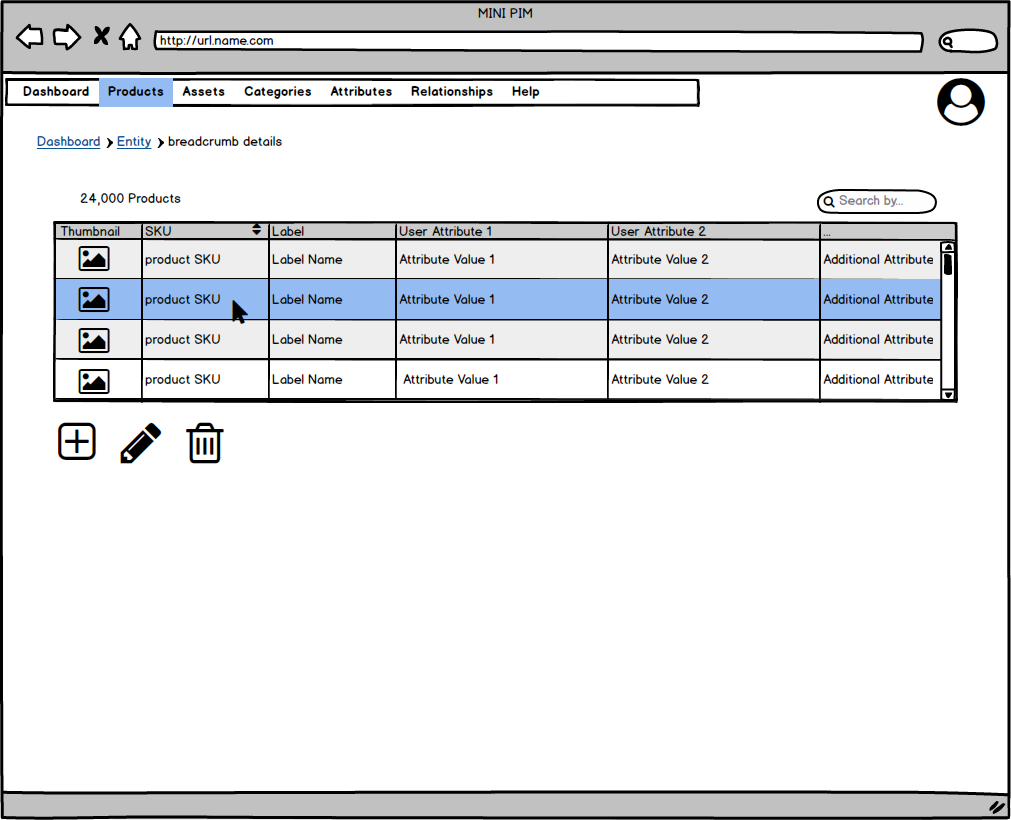
\includegraphics[width=1\linewidth]{mockups/RF2.X_MostrarProducto(Desde Listado).png}
    \caption{Mostrar Producto}
   \end{figure}
\vspace{1.0cm}
\numberedsubsection{Bocetos}
\begin{figure}[H]
    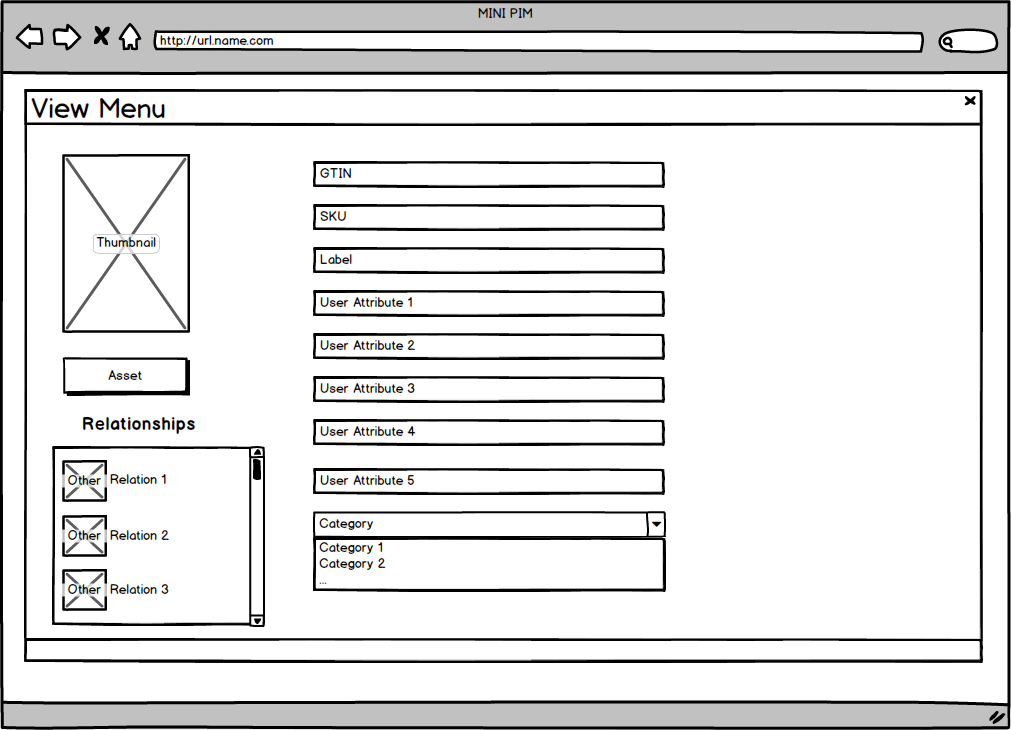
\includegraphics[width=1\linewidth]{mockups/RF2.X_MostrarProducto(Menu visualizacion).png}
    \caption{Mostrar Producto}
   \end{figure}
\vspace{1.0cm}


\newpage %Inicia en una nueva página otro caso de uso